%!TEX root = ../article.tex

\section{Related Work}
\label{chapter:relatedWork}

A \textit{programming system} has two fundamental parts: the \textit{programming language} that users should know to create a program, and the \textit{programming environment} that is used to write and test programs. Undoubtedly, both parts are equally important to build a program and understand it. However the boundaries between these components can be blurred, for this reason, the related work goes beyond programming environments including also programming languages and their design aspects.

%%%%%%%%%%%%%%%%%%%%%%%%%%%%%%%%%%%%%%%%%%%%%%%%%%%%%%%%%%%%%%%%%%%%%%%%%%%%%%%%%%%%%%%%%%%%%%%%%%%%%%%%%
\subsection{Processing}
\label{subsec:processing}
Processing~\cite{Reas2006} is a programming language and environment designed to teach programming in an optic context. Processing has become popular among students, artists, designers, and architects because it acts as a tool to get non-programmers started with programming through instant visual feedback.

The Processing programming language is built on top of Java, but it removes much of the verbosity of Java to make the syntax accessible to novices. The language provides simple access to external libraries, such as OpenGL, through single entry points, such as \texttt{setup} and \texttt{draw}. Therefore, this allows novices to quickly prototype, learn fundamental concepts of programming, and, eventually, gain the basis to learn other programming languages.

The programming environment contains a simple text editor, a text console to present errors, and a run button. The run button compiles the Processing code and executes it. Moreover, in the default mode, the program result is displayed in a 2D graphical window, the render can be configured to present the result in 3D, or other sophisticated methods using \textit{shaders} to recur directly to the graphic board.

Actually, with a few changes, the Processing code can be exported as an application for different platforms, such as Java, JavaScript, and Android. For example, to export a Processing program for JavaScript, it is only necessary to create a HTML page and include the Processing code as a script of this page. Then the Processing code will be automatically parsed and translated to JavaScript. To maintain the usual render capabilities of a Processing program, it will use the HMTL5 canvas with WebGL.

The popularity of Processing is explained by the benefits of these features, besides of being a domain-specific language. However, it has drawbacks that can discourage its use, such as the following:

\begin{itemize}
  \item \textit{Weak metaphor}. The Processing programming language, by contrast with the above systems, has none strong metaphors that allow the programmer to translate his experiences as a person into programming knowledge. 

  \item \textit{Poor decomposition}. Processing discourages the elementary approach to solving a complex problem by breaking it into simpler problems because drawing and input events link to single entry points. Thereby the behavior of submodules must be tangled across these global functions, making it difficult to achieve clean decomposition.

  \item \textit{Poor recomposition}. Processing discourages combining two programs. The designer cannot just grab and use part of other programs because variables must be renamed or manually encapsulated, and the \texttt{draw} and mouse functions must be woven together. Even worse, Processing has global modes which alter the meaning of the function arguments. For example, two Processing programs can specify its colors in different modes and each mode has its proper purpose of \texttt{fill} function arguments. Combining those programs will be almost impossible. 

  \item \textit{Weak readability}. The syntax of a Processing program represents a significant barrier for reading. For example, the function which draws an ellipse on screen is written as \texttt{ellipse(50,50,100,100)}. The reader must look up or memorize the meaning of every single argument.

  \item \textit{Fragile environment}. The programming environment is fragile because it does not attempt to solve any of the above issues related to the language and its implementation.
\end{itemize}

%%%%%%%%%%%%%%%%%%%%%%%%%%%%%%%%%%%%%%%%%%%%%%%%%%%%%%%%%%%%%%%%%%%%%%%%%%%%%%%%%%%%%%%%%%%%%%%%%%%%%%%%%
\subsection{DesignScript}
\label{subsec:designscript}
DesignScript~\cite{aish2012designscript} is a programming language and environment designed to support \gls{gd} with textual methods. It is mainly used by architects and designers to generate geometric models using a script. Then when the script executes it creates new models in a \gls{cad} tool. DesignScript is an AutoDesk\footnote{\texttt{http://www.autodesk.com/products}} product initially proposed to be used within AutoCAD, nowadays it provides the same functionality on top of Revit, another AutoDesk product used for \gls{bim}. In short, a \gls{bim} model is similar to a \gls{cad} model, but it covers more than just geometry. It also includes spatial relationships, properties of building components, such as manufacturers' details.

The programming language is an associative paradigm. The variables are abstract types that can represent numeric values or geometric entities. These variables are in a graph of dependencies. When a change in a variable occurs it forces the re-evaluation of the graph, as shown in Figure~\ref{fig:designscript}, consequently variables has always updated values. This feature is useful, especially in a modeling environment, because it provides continuous feedback to the designer as the model is modified.

\begin{figure}[!h]
  %\vspace{-5pt}
  \centering
    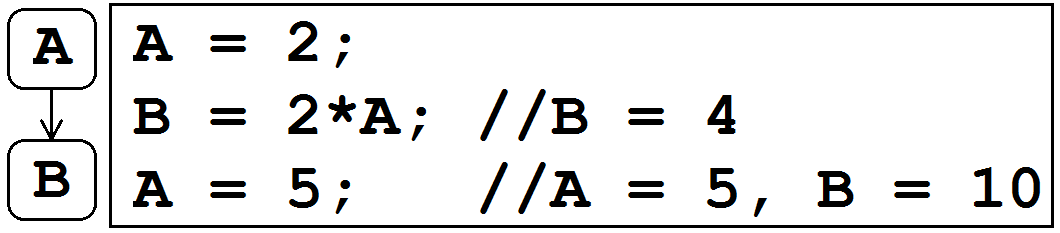
\includegraphics[width=0.3\textwidth]{images/designscript}
  %\vspace{-20pt}
 \caption{Associative interpretation}  
  %\vspace{-20pt}
    \label{fig:designscript}
\end{figure}

The DesignScript's programming environment provides a text editor, an interpreter, and a simple debugger. The language interpreter executes each time that the designer clicks on the run button. Then all the script is interpreted, and its result produces geometric entities rendered in the \gls{cad}. The continuous feedback feature works only in debug mode because, in this way, the script is interpreted line by line. Thus, each update to a variable will change its dependencies and will recompute the model. However, in debug mode the code cannot be edited, so this feature is worthless during code editing.

In the DesignScript's debug mode, users can inspect the variable values by adding \textit{watchers} to them. A watched variable is showed in a particular tab, as shown in Figure~\ref{fig:designscript}. In case the variable represents a geometric model, the own design will be highlighted in the \gls{cad} when the variable is selected. It creates a certain \textit{traceability} between patterns in the \gls{cad} and code in the editor. In this way, the user is able to correlate which model a variable corresponds. However the inverse, starting to form the model and finding the correspondent variable, is unsupported.

DesignScript also supports a typical mechanism of \textit{live} programming environments: the sliders. The sliders are widgets which facilitate giving new values to the program input. This way, designers can create new models reacting to these changes. However, in the DesignScript's sliders, the changes are reflected in the models only when the programmer leaves the slider. Until then, the designer should imagine how the model would be with the new value, which is completely against the purpose of sliders.

Moreover the DesignScript language, despite being presented as pedagogic, has some drawbacks. It does not carry any manly metaphor which helps beginners start with the language. Additionally, the associative paradigm represents a barrier for sharing code: it discourages the recomposition of modules because new modules can change the previous one. The environment provides poor mechanisms that help people to find bugs in the code, and finally,  DesignScript is confined to produce geometry in a single \gls{cad} tool.
%%%%%%%%%%%%%%%%%%%%%%%%%%%%%%%%%%%%%%%%%%%%%%%%%%%%%%%%%%%%%%%%%%%%%%%%%%%%%%%%%%%%%%%%%%%%%%%%%%%%%%%%%
\subsection{Monkey} 
\label{subsec:monkey}
Monkey\footnote{\texttt{http://wiki.mcneel.com/developer/monkeyforrhino4}} is a programming environment designed to support \gls{gd}. Like DesignScript, Monkey is used to edit, debug and interpreter scripts. However, Monkey uses RhinoScript as its programming language and Rhinoceros3D\footnote{\label{fnote:rhin}\texttt{https://www.rhino3d.com}} (or Rhino for short), a lighter \gls{cad} than AutoCAD, to generate the geometric models.

Monkey is implemented as a \texttt{.NET} plugin for Rhino4 and provides a programming environment to write and debug scripts. The RhinoScript is based on Microsoft's VBScript language (a descendant of BASIC), and like VBScript, it is a weakly typed language. One of the major drawback with this language is the fact that users must beware with the data passed in their functions at all time because RhinoScript can accidentally cast variables into inappropriate types. Therefore, it creates errors difficult to find, especially for people who are learning to program.

Monkey is based on general-purpose programming environments. It provides typical features of those environments, namely syntax highlighting, auto-completion, and error highlighting. The organization of code into trees is also similar. However, the programming environment and language do not provide any well-designed feature which helps beginners to start with programming. The offered features are based on general-purpose systems, instead of being tailored for \gls{gd}.
%%%%%%%%%%%%%%%%%%%%%%%%%%%%%%%%%%%%%%%%%%%%%%%%%%%%%%%%%%%%%%%%%%%%%%%%%%%%%%%%%%%%%%%%%%%%%%%%%%%%%%%%%
\subsection{Rosetta}
\label{subsec:rosetta}
Rosetta~\cite{lopes2011portable} is a programming environment designed to support \gls{gd} that is based on DrRacket~\cite{findler2002drscheme}. Like Monkey, Rosetta provides its environment detached from the \gls{cad}. Rosetta is a step forward from the previous systems, because it solves the portability problem among \gls{cad} tools. In Rosetta a \gls{gd} program can be written in various programming languages (frontends) and the geometric models can be rendered by different \glspl{cad} (backends). As a result, designers are free to write their programs in their selected frontend which, upon execution, will generate the same geometry for the various backends.

Rosetta has been used to teach programming in architecture courses. Tailored to this end, Rosetta uses DrRacketas its programming environment. The DrRacket environment serves some functions, but the most important are that the student can start immediately to learn to program. For instance, the environment is set up with just three lines of code.

The Racket language is also an advantage of Rosetta's environment because it encourages the use of the scientific paradigm for writing algorithms. In this way, students that learn simple programming techniques, such as recursion, can create robust models. Additionally, as the students progress, new programming languages are also available to learn, such as JavaScript, Python, Processing, and so on.

The Rosetta's environment provides some interesting tools for \gls{gd}, such as a programming flow tracer, similar to the DesignScript's watcher. It highlights models in the \gls{cad} upon selection of expressions, it also supports the inverse, selecting the mode in the \gls{cad} and shows the expression in the code editor. Another interactive tool is the slider, an attempt to provide immediate feedback to the designers. It uses the DrRacket slider, associating the slider callback to the function that generates the entire model, so each time the slider change a new model will be created. However, this process must be performed manually.

Undoubtedly Rosetta's environment goes further than the textual environments for \gls{gd} presented in this report. However, it presents some drawbacks which may discourage the learning in general. Beginning with the usual programming language: Racket. The syntax of a Racket program represents a significant barrier for reading. For instance the function which draws a circle in Rosetta is written as \texttt{(circle (xy 0 0) 1)}. The reader must lookup or memorize every argument. Using the Rosetta's documentation the reader will spend even more time because it is in a book mixed with architecture topics.
%%%%%%%%%%%%%%%%%%%%%%%%%%%%%%%%%%%%%%%%%%%%%%%%%%%%%%%%%%%%%%%%%%%%%%%%%%%%%%%%%%%%%%%%%%%%%%%%%%%%%%%%%
\subsection{Grasshopper}
\label{subsec:grasshopper}
Grasshopper\footnote{\texttt{http://www.grasshopper3d.com/}} is a programming language and environment designed to support \gls{gd} using a visual language. Grasshopper provides an alternative way to programming. By definition, it is a bi-dimensional representation consisting of iconic components that can be interactively manipulated by the user according to some spatial grammar~\cite{myers1990taxonomies}. For example, the boxes in Figure~\ref{fig:grass} are components which receive the input (left ports) perform some operations and return the output (right port). The components link to other elements establishing a \textit{dataflow} paradigm where the input of an element is the output of another.

\begin{figure}[!htbp]
%\vspace{-5pt}
  \centering
  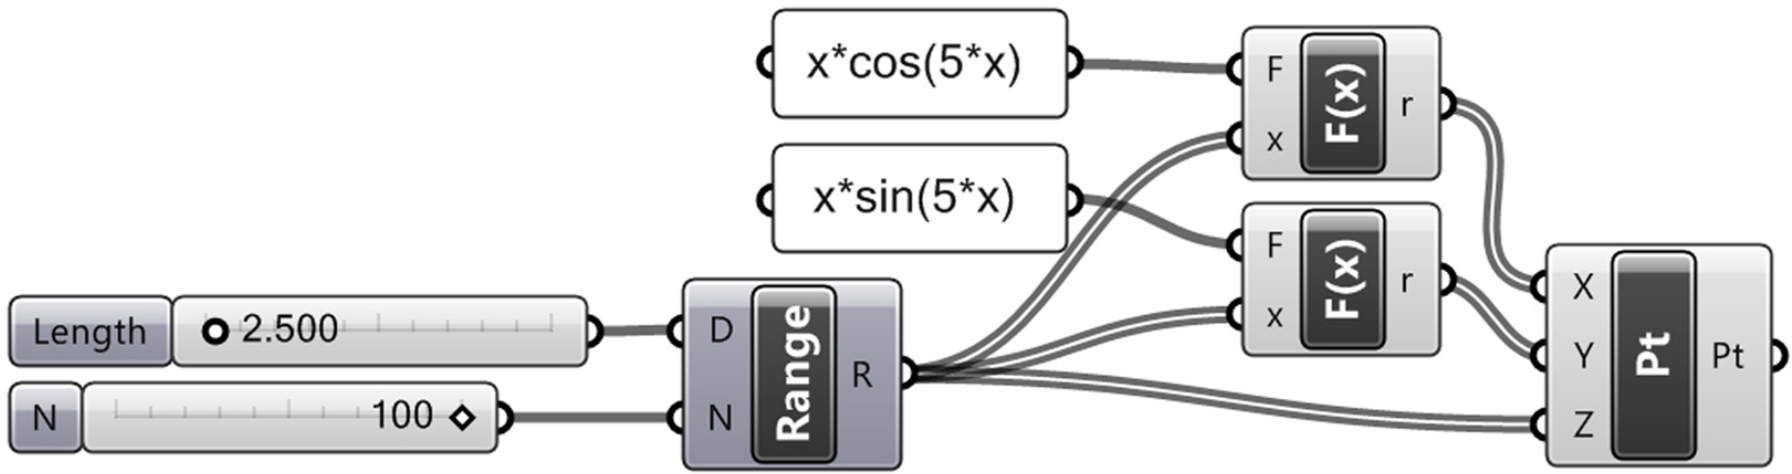
\includegraphics[width=0.4\textwidth]{images/grasshopper}
  %\vspace{-5pt}
    \caption{A program in Grasshopper that computes the 3D coordinates of a conical spiral. Each time the left sliders are dragged a new coordinate is calculated.}
  \label{fig:grass}
  %\vspace{-10pt}
\end{figure}

Like Monkey, Grasshopper is implemented as a \textit{plugin} for Rhino$^{\ref{fnote:rhin}}$. However, Grasshopper tailors the Rhino's environment with specific \gls{gd} tools. These tools are state of the art because they implement important principles for design models, such as the following:

\begin{itemize}
 \item \textit{Get immediate feedback}. As the user interacts with the components, by adding and connecting them, the result reflects immediately in the \gls{cad} model. It facilitates the design conception because the user's intentions are immediately visible. 
 \item \textit{Facilitate program input}. To facilitate the process of design exploration, Grasshopper provides sliders which connect at the component input. Dragging the slider causes a change propagation through components. The components are re-executed with the new slider value. Combined with the above feature new models are generated immediately.
 \item \textit{Correlate the program with the generated elements}. Like DesignScript's watcher, by selecting a component, its geometry is highlighted in the \gls{cad}. It allows designers to understand a program better by figuring out the roles for each element.
 \item \textit{Show comparisons between models}. Grasshopper provides a special component that, when connected to the output of another component, replicates the geometry. This mechanism is useful for design exploration because it maintains in the \gls{cad}'s background an old replica of the changed geometry. It adds a context at each change so that the designer can compare the result of his change in the new geometry based on the old one.
\end{itemize}

Mainly, the Grasshopper interactivity depends on the immediate feedback tool. However, this tool will never scale for arbitrarily complex programs because the \gls{cad}'s render is not designed to process the massive amount of information generated by \gls{gd} methods. Other systems, such as DesignScript and Rosetta, improve this problem by sidestepping most of the functionality of traditional \gls{cad} tools and focusing only on the generation and visualization of geometric models. These systems provide a backend based on OpenGL that is independent of a full-fledged \gls{cad} application, but, in Grasshopper, there is no so backend.

Moreover, the traceability among components is just in one direction. From the designer perspective, it would be more useful start from the geometry and find which component implements it, but it is unsupported. However, despite the usefulness of model comparison in design exploration, this feature is also unsupported.
%%%%%%%%%%%%%%%%%%%%%%%%%%%%%%%%%%%%%%%%%%%%%%%%%%%%%%%%%%%%%%%%%%%%%%%%%%%%%%%%%%%%%%%%%%%%%%%%%%%%%%%%%
\subsection{Dynamo}
\label{subsed:dynamo}
Dynamo\footnote{\texttt{http://dynamobim.com/}} is a programming language and environment designed to support \gls{gd}. Like Grasshopper, Dynamo provides an alternative way to programming. However Dynamo, like DesignScript, is implemented on top of Revit, an Autodesk product for \gls{bim}.

Dynamo provides a set of tools similar to Grasshopper, particularly a searching table, which provides quick access to the primitives of the language, such as the components and widgets. This feature encourages designers to explore the available parts and try current components.

In general, Dynamo and Grasshopper are programming environments and visual languages popular among novices in programming. The smooth learning curve and perhaps the style of the \gls{ui} elements are attractive for beginners. However as the visual programs become broad and complex, it requires more time to understand, maintain, and adapt to new requirements, than the textual programs as showed in~\cite{leitao2011programming}. Despite spending more time and effort to learn a textual programming language, the learners have their time quickly recovered once the complexity of the design task becomes sufficiently large.
%%%%%%%%%%%%%%%%%%%%%%%%%%%%%%%%%%%%%%%%%%%%%%%%%%%%%%%%%%%%%%%%%%%%%%%%%%%%%%%%%%%%%%%%%%%%%%%%%%%%%%%%%

In the surveyed systems, the typical representation of code is textual. This representation is typically static and, to be understood, requires the reader to know the vocabulary of the programming language. For a novice, it is simply a barrier to learning. On the other hand, the representation of programs as graphical components or mathematical forms lowers this barrier, because the information is visually more perceptible, but it becomes incomprehensible as the program grows.